\documentclass[a4paper, 11pt]{article}
\usepackage[english]{babel}
\usepackage{appendix}
\input{"/media/alessandro/OS/Users/ale57/Documents/1. universita'/ANNO IV (2019-2020)/second semester/header.tex"}

\begin{document}

\title{NNDL: Homework 1 \\ Supevised Deep Learning}
\author{Alessandro Lovo}
\maketitle

\section{Introduction}
  This homework consists in applying supervised deep learning to two tasks: a regression task consisting in approximating a scalar function of a scalar variable and a classification task that is recognizing the handwritten digits of the MNIST dataset. For the regression task a fully connected network (FCN) will be used, while for the classification task both a fully connected but most importantly a convolutional network (CNN) will be tested. In both cases different architectures, optimization and visualization techniques and hyperparameter search will be tried.

  \subsection{General framework}
    Both tasks rely on a framework of python classes that unfolds as follows:
    \begin{itemize}
      \item \textbf{Net}: class inheriting from \emph{torch.nn.Module} that contains the actual neural network with a specific architecture.
      \item \textbf{Evolver}: class for handling the training and validation of a \emph{Net}. In this class there is a check at the end of every training epoch to interrupt the learning process. To implement early stopping one just needs to inherit from the \emph{Evolver} class and specify that check condition. In particular the learning process stops if the validation loss isn't decreasing after \emph{patience} number of epochs.
      \item \textbf{KFoldCrossValidator}: class for performing k fold cross validation on a particular set of hyperparameters.
    \end{itemize}

\section{Regression task}
  \subsection{Basic solution}
    The data for this task consists in 100 points for training, arranged in such a way to leave two 'gaps' (fig \ref{fig:r:basic} b), and 100 test points that fill the gaps, allowing to test how good the net is in generalizing its learning.

    As a basic solution I implemented a two layered FCN with 128 neurons per hidden layer, the sigmoid as activation function and trained it for 2000 epochs using the Adam optimizer with learning rate set to $10^{-3}$ and a batch size of 10 datapoints. The loss function used is the mean square error (MSE) and 10\% of training data is used for validation. In fig \ref{fig:r:basic} are shown the results and one can see that the model is, unsurprisingly, not very good. In particular the validation loss started to increase just after 500 epochs and still there is some underfitting on the training data.
    To solve these issues one requires both a more complex model and some regularization techniques.

    \begin{figure}
      \centering
      \subfloat[]{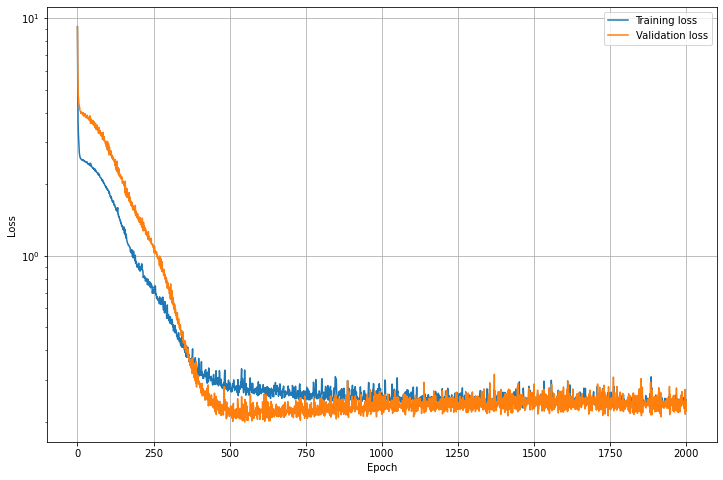
\includegraphics[width=0.4\textwidth]{img/regression/basic_loss.png}} \quad
      \subfloat[]{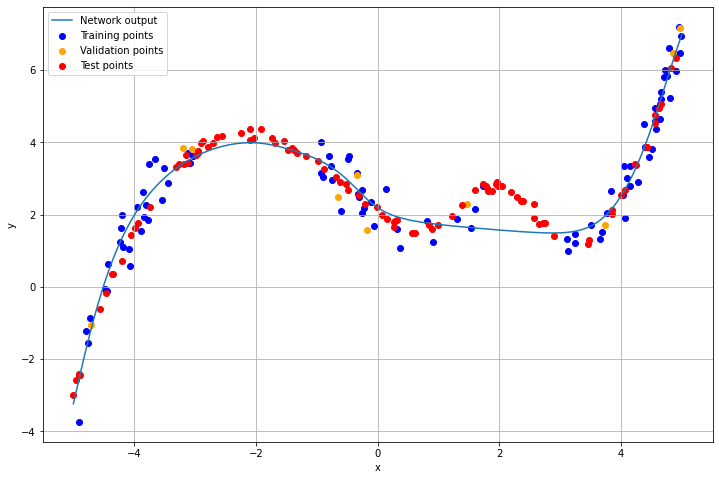
\includegraphics[width=0.4\textwidth]{img/regression/basic_plot.png}}
      \caption{Results of the basic solution: training and validation loss as a function of epoch number (a) and Output of the trained network compared with training, validation and test datapoints (b).}
      \label{fig:r:basic}
    \end{figure}

  \subsection{More advanced methods}
    Since there is quite few training data, the result is highly dependent on the train-validation split, so to improve this in the followinig every set of hyperparameters will be tested with a 5-fold setup.
    Also it is worth introducing the early stopping in order to be able to increase the maximum number of epochs (for example to $10^4$) without worrying about overfitting. In practice this is implemented creating a checkpoint for the network every time the validation loss reaches a new minimum; if there is no new minimum after \emph{patience} epochs, learning stops and the net is reverted back to the last checkpoint.
    At this point one can test different architectures (2, 3 or 4 layers with or without dropout and different activation functions: Sigmoid, ReLU or Tanh) and optimization procedure (momentum for the SGD optimizer and weight decay for the Adam optimizer).

    Since the number of combinations of hyperparameters rockets, it would be better to rule out some of these possibilities.
    In particular Adam yields reliably better results than SGD with momentum, and also the Sigmoid activation function frequently yields a heavy underfitting. Also having a too small training batch size makes the learning process very unstable and on average a 4-layered network performs better than a 3-layered one. So, the architecture to be tested now is a network with 4 hidden linear layers, where the second and third one are followed by a dropout layer.

    At this points the remaining degrees of freedom are the following, and for each of them I provided a list of possibilities to be tested in a random search
    \begin{itemize}
      \item the number of neurons in each layer: [8, 16, 32, 64, 128, 256]
      \item dropout probabilities: [0, 0.15, 0.35, 0.5]
      \item activation function: [Tanh, ReLU]
      \item learning rate and weight decay for the Adam optimizer: respectively [$10^{-4}$, $5\cdot10^{-4}$, 0.001, 0.005, 0.01, 0.05] and [0, $10^{-5}$, $5\cdot10^{-5}$, $10^{-4}$, $5\cdot10^{-4}$, 0.001]
      \item patience parameter for the early stopping: [100, 200, 300, 400]
      \item training batch size: [20, 30, 40, 50]
    \end{itemize}
    To speed up the random search I also implemented trial pruning, i.e., if in one of the first three folds the validation loss is above 0.4, the remaining folds are not computed, directly testing the next hyperparameter combination and thus saving time.

  \subsection{Results}
    After 65 non pruned iterations of the random search the best hyperparameter combination is found in hidden layers with 32, 128, 64, 256 neurons, with 0.5 dropout probability after the second layer and Tanh as activation function, trained with learning rate of 0.001, no weight decay, a train batch size of 30 and patience of 400, resulting in an average validation loss of 0.227.
    Since during the random search networks weren't saved, now I performed a final 5-fold run with the best hyperparameters and select the best of the five nets obtaining the results in fig \ref{fig:r:best}. If one compares with the basic solution this one doesn't seem much better, however by comparing the two test losses, the best net performs quite better, proving to be more able to generalize than the basic one (tab \ref{tab:r:losses}).

    If one visualizes the weight histogram of the weights can see that, due to the lack of weight decay, the weights are not very peaked around 0, and also the distribution is broader on the second layer, where dropout was applied. On the other hand the activation profiles are not very interpretable (fig \ref{fig:r:visualization}).

    \begin{figure}
      \centering
      \subfloat[]{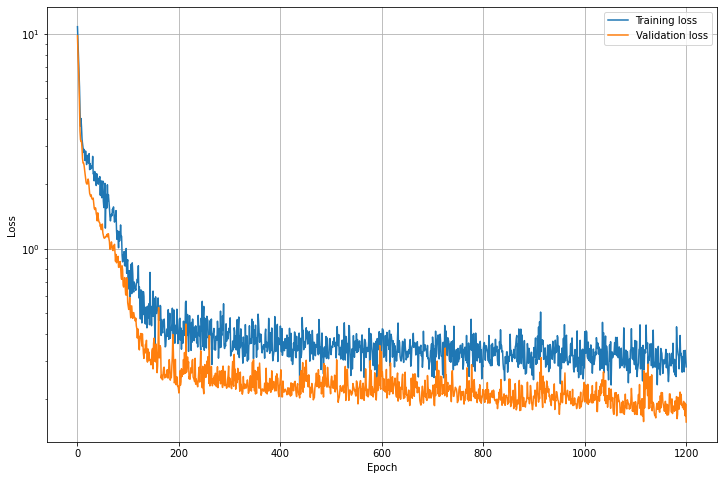
\includegraphics[width=0.4\textwidth]{img/regression/best_loss.png}} \quad
      \subfloat[]{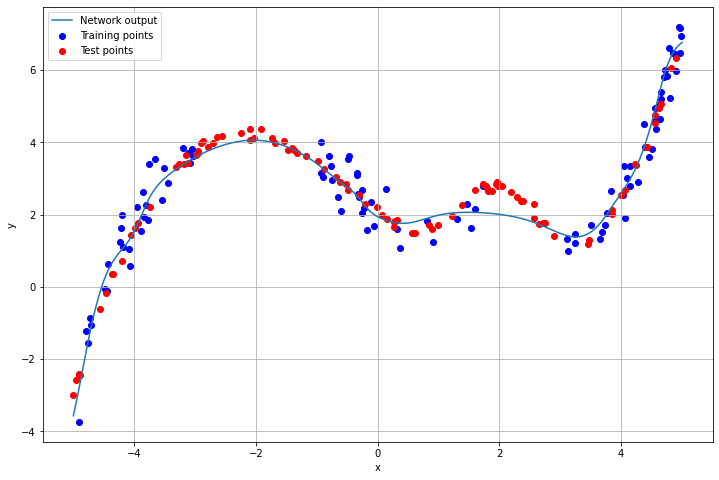
\includegraphics[width=0.4\textwidth]{img/regression/best_plot.png}}
      \caption{Results of the best network: training and validation loss as a function of epoch number (a) and Output of the trained network compared with training/validation in blue and test datapoints in red (b).}
      \label{fig:r:best}
    \end{figure}

    \begin{table}
      \centering
      \begin{tabular}{c|ccc}
        Net & Training loss & Validation loss & Test loss \\
        \midrule
        Basic & 0.2418 & 0.2375 & 0.3417 \\
        Best & 0.3008 & 0.1822 & 0.1216
      \end{tabular}
      \caption{Comparison of the losses of the basic and best net.}
      \label{tab:r:losses}
    \end{table}

    \begin{figure}
      \centering
      \subfloat[]{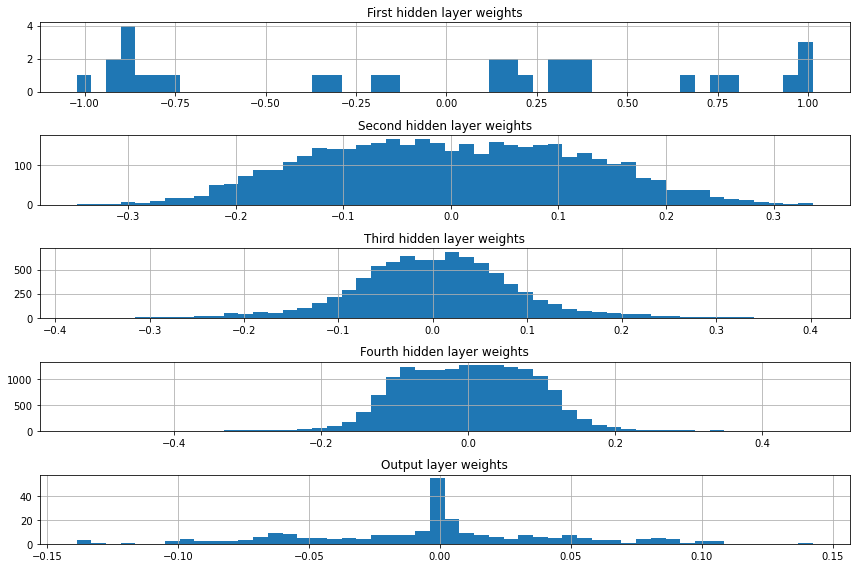
\includegraphics[width=0.4\textwidth]{img/regression/best_w.png}} \quad
      \subfloat[]{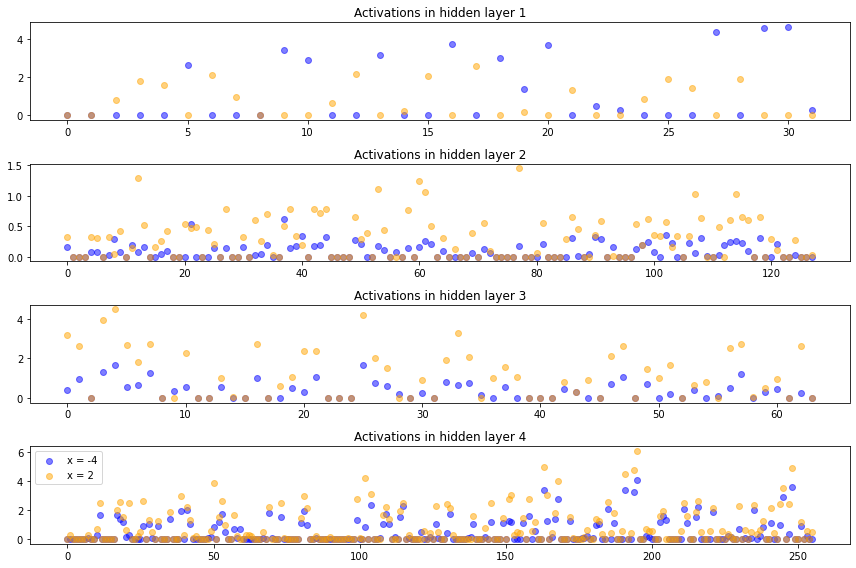
\includegraphics[width=0.4\textwidth]{img/regression/best_act.png}}
      \caption{Visualization of the weights and activations of the best net.}
      \label{fig:r:visualization}
    \end{figure}


\section{Classification task}
  \subsection{Basic solution}













\end{document}
